\documentclass{article}
\usepackage[top=0.2in, bottom=0.1in,left=1.5cm,right=1.5cm]{geometry}
\usepackage{graphicx}
\usepackage{background}

\SetBgScale{1}
\SetBgAngle{0}
\SetBgColor{black}
\SetBgContents{\rule{.5pt}{\paperheight} \rule{.5pt}{\paperheight} 
\qquad \qquad \qquad \qquad \qquad \qquad \qquad \qquad \qquad 
\qquad \qquad \qquad \qquad \qquad \qquad \qquad \qquad \qquad 
\qquad \qquad \qquad \qquad \qquad \qquad \qquad \quad \quad \, \rule{.5pt}{\paperheight} \rule{.5pt}{\paperheight}
}

\begin{document}

\hrule  
\vspace{0.1in}
\includegraphics[width=4cm]{chalk_logo.png}
\Huge{\quad \textbf{CB01 - DC Hbridge \quad \quad} \emph{rev1}} 
\vspace{0.05in}
\hrule 
\vspace{0.05in}


\mbox{
\begin{minipage}[t]{0.4\linewidth}
\vspace{0pt}
\large
\textbf{Features and Benefits}
\normalsize
\begin{itemize}
\item High current(5A) DC motor drive
\item Multiple protection schemes
\item Current sense via space saving I2C
\item I2C reports current, voltage, and power.
\item Alert pin to alert of overcurrent conditions.
\item Requires only a single battery voltage (7-30V).
\item Diagnostics output provided over 3 pins.
\item has an low current sleep modes.
\item capable of 100\% duty cycle with a unique top off charge pump.
\end{itemize}
\end{minipage}

\vrule
\vspace{0.3in}

\begin{minipage}[t]{0.5\linewidth}
\vspace{0pt}
\large{\textbf{Descritpion}} 
\\

\normalsize
CB01 is a full-bridge controller with externaal power MOSFETs. It is specifically designed to drive our high power brush DC motors. \\
This part is specifically designed to be extremely modular. It is completely enclosed and does not require any external components. This makes the module extremely easy to test, use and develop for.\\
We have implemented an extremely flexible modes of control. This module can be driven with fast or slow decay modes with either diode or synchronous rectification. There is deadtime set at 1 microsecond between turn on of low side mosfets and turn off of high side mosfets.\\
Integrated diagnostics provide warnings of undervoltage, overtemperature [only on controller], overcurrent, overvoltage, power bridge faults and short circuits. The CB01 is provided in a module 1.2"x1.7" with logical pinpouts and motor screws.
\end{minipage}
} %end mbox
\\
\hspace{0.3in}
\hrule
\hspace{0.3in}
\begin{center} 
\large{\textbf{Typical Application}}
\end{center}
\begin{center}
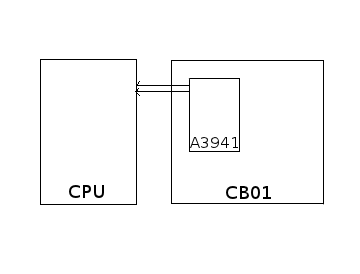
\includegraphics[width=6in]{cb01_typical.png}
\end{center}
\hrule
\newpage
\large{\textbf{Electrical Characterestics}} \\
%page 2!
\begin{center}
\begin{tabular}{|l | l |c| c|c|c|c|}
\hline
Characteristics & Symbol &Test Conditions & Min & Typ & Max & Units \\ \hline
Functional Voltage& $V_{bb}$& & 7&12&35&V \\ \hline 
Output Current & $I_{motor}$ & NOT TESTED YET& -5 & 0& 5 &A \\ \hline
MOSFET resistance & $Rds_{on}$  & Datasheet values& & 7 & 8.5 & mOhms\\\hline
\hline
\end{tabular}
\end{center}

\end{document}


